\documentclass[a4paper, 12pt, oneside]{scrbook}

\usepackage[backend=bibtex]{biblatex}
\usepackage[ngerman]{babel}		
\usepackage[T1]{fontenc}	  	
\usepackage[utf8]{inputenc}
\usepackage[hidelinks]{hyperref}
\usepackage{graphicx}
\usepackage{epstopdf}
\usepackage{float}
\usepackage{acronym}
\usepackage{booktabs}
\usepackage{caption}
\usepackage{csquotes}
\usepackage{fancyhdr}
\usepackage{url}
\usepackage{pdfpages}
\usepackage{mathtools}
\usepackage{float}
\usepackage{array}
\usepackage{tabularx}
\usepackage{etoolbox}

\renewcommand*{\headfont}{\normalfont}
\renewcommand*{\multicitedelim}{\addsemicolon\space}
\renewcommand*{\arraystretch}{1.5}
\renewcommand{\headsep}{15pt}

\setlength{\parskip}{1.5ex}

\renewcommand*\chapterpagestyle{fancy}

\input{header_footer.tex}
\renewcommand{\title}{Entwicklung einer Lösung des Traveling Salesman Problem mithilfe der parallelisierten Optimierung durch den Ameisenkolonie-Algorithmus}
\renewcommand{\author}{Viktor Rechel}
\newcommand{\doctype}{Studienarbeit}

\newcommand{\Matrikelnummer}{6335802}
\newcommand{\Kurskuerzel}{Inf15A}
\newcommand{\Company}{Fujitsu TDS GmbH}
\newcommand{\Gutachter}{Dr. Carsten Müller}

\bibliography{bibliography}

\begin{document}
\frontmatter
\begin{titlepage}

\vspace{10mm}

\begin{center}
	\vspace{5mm}
	
	\huge \title
	
	\vspace{14.2pt}
	
	\large \doctype \\
	\small im Rahmen der Vorlesung "Datenbanken 2 - Business Intelligence"
	
	\vspace{42.6pt}
	
	\small des Studienganges Angewandte Informatik an der \\
	\large Dualen Hochschule Baden-Württemberg Mosbach
    
    	\vspace{14.2pt}
	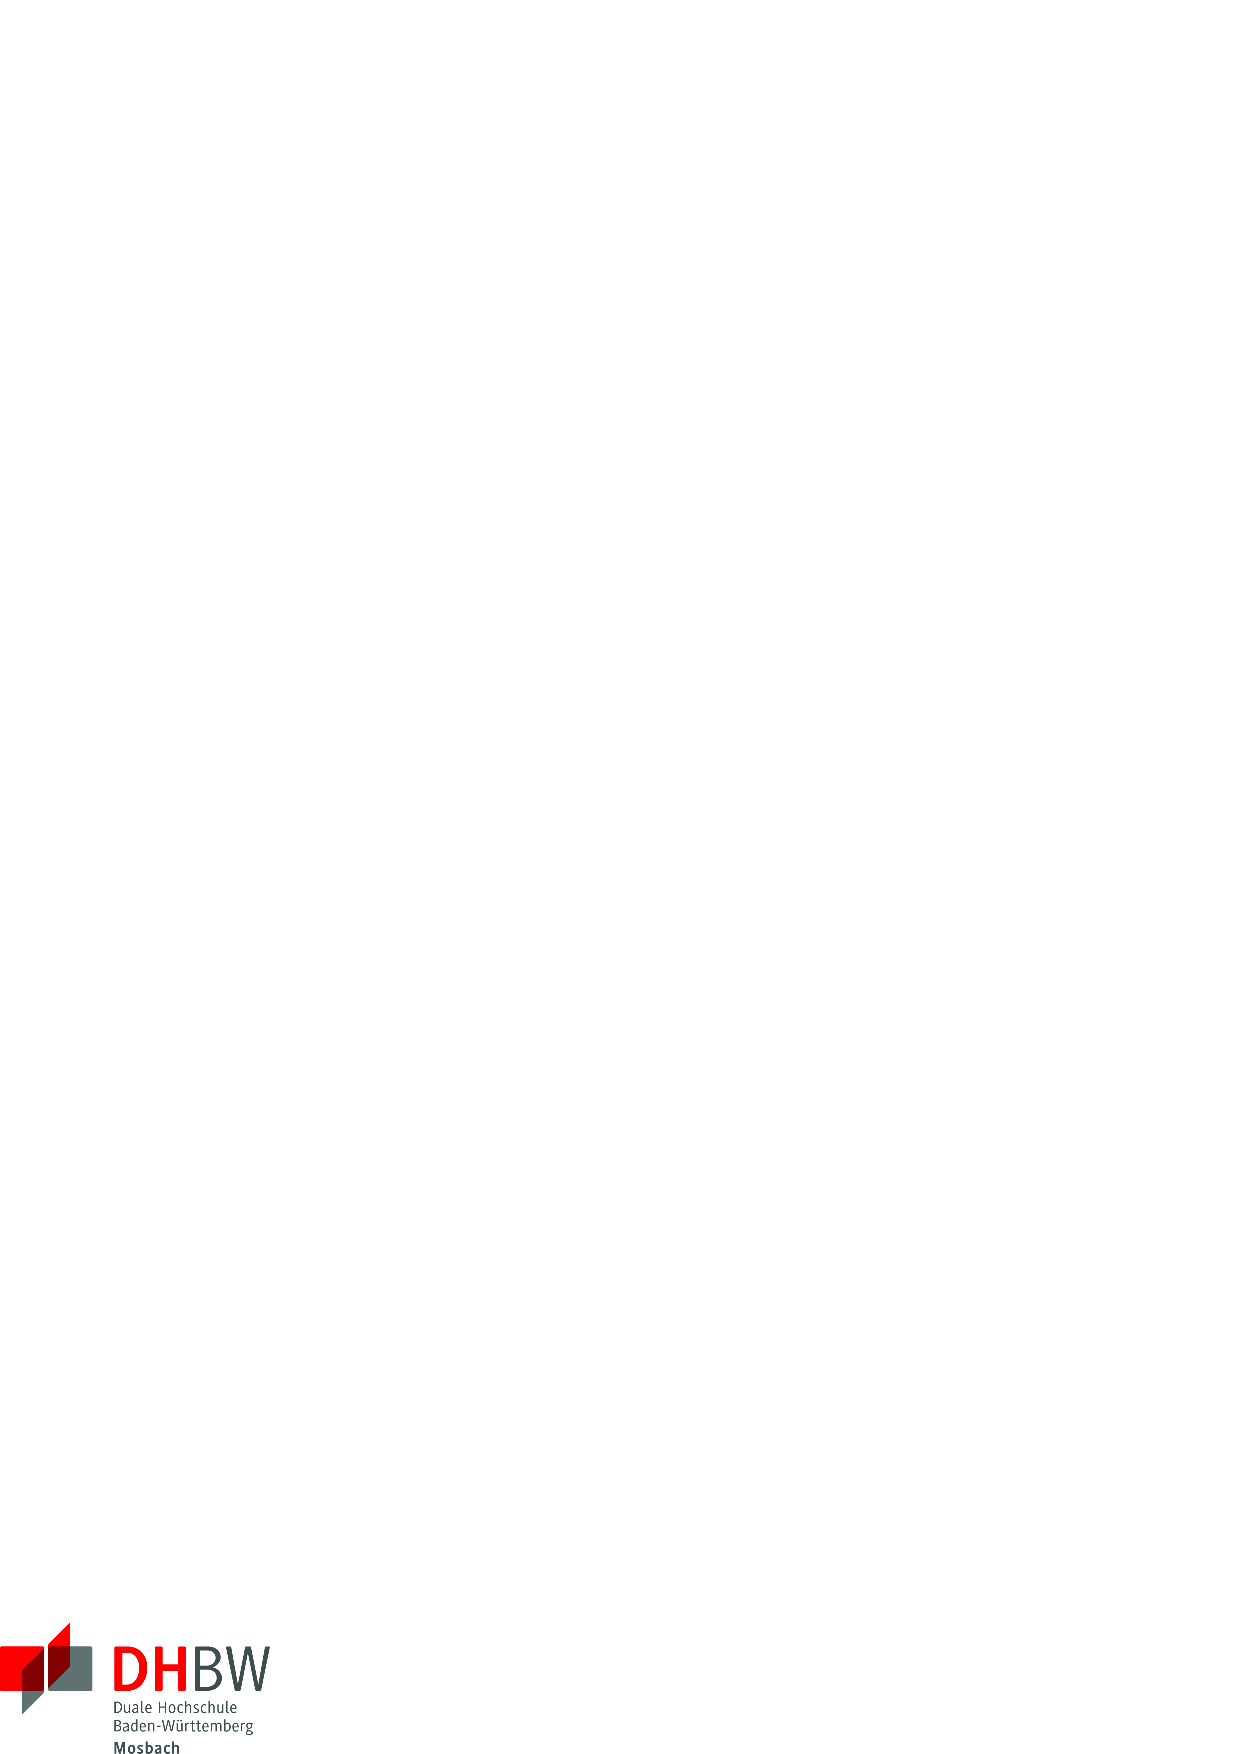
\includegraphics[width=4cm]{images/logo.jpg}
	\vspace{100pt}
   	\hspace{35pt}
	
	\small von \\
	\large \author
\end{center}

\vspace{98.6pt}

\begin{table}[h]
    \centering
    \begin{tabular}{ll}
        \small Bearbeitungszeitraum                 & 12 Wochen                     \\
        \small Matrikelnummer, Kurs                & \Matrikelnummer, \Kurskuerzel    \\
        \small Ausbildungsfirma                     & \Company       \\
        \small Gutachter der Dualen Hochschule      & \Gutachter        \\
    \end{tabular}
\end{table}

\vspace{49.7pt}

\fancypagestyle{empty}{
  \fancyhf{}
  \fancyfoot[C]{\today}
}

\end{titlepage}
\addchap*{Ehrenwörtliche Erklärung}

\fancyhead{} % clear all header fields
\fancyhead[L]{}
\fancyhead[C]{}
\fancyhead[R]{Ehrenwörtliche Erklärung}
\fancyfoot{} % clear all footer fields
\fancyfoot[L]{Viktor Rechel}
\fancyfoot[C]{}
\fancyfoot[R]{\thepage}

Ich, \author, versichere hiermit, dass ich meine Studienarbeit mit dem Thema
\begin{quote}
	"\title"
\end{quote}
selbstständig verfasst und keine anderen als die angegebenen Quellen und Hilfsmittel benutzt habe, wobei ich alle wörtlichen und sinngemä\ss en Zitate als solche gekennzeichnet habe.

Ich versichere zudem, dass die eingereichte elektronische Fassung mit der gedruckten Fassung
übereinstimmt.

\vspace{3cm}
%\hspace{2cm} Ort, Datum \hfill Unterschrift \hspace{2cm}
\ort, den \today \hspace{4cm}
\begin{tabular}{r}\hline
	\rule{1.5cm}{0pt}
	\author
\end{tabular}


%\noindent
%\begin{tabular}{l r}
%	\ort, den \today &
%	\begin{tabular}{@{}l@{}}\hline
%		\rule{0pt}{2ex}
%		Hans Lümmelmeier
%	\end{tabular}
%\end{tabular}


\addchap*{Abstract}
\thispagestyle{fancy}
\renewcommand{\headrulewidth}{0.5pt}
\renewcommand{\footrulewidth}{0.5pt}

\fancyhead{} % clear all header fields
\fancyhead[L]{}
\fancyhead[C]{}
\fancyhead[R]{Abstract}
\fancyfoot{} % clear all footer fields
\fancyfoot[L]{Viktor Rechel}
\fancyfoot[C]{}
\fancyfoot[R]{\thepage}

I am an abstract
\addchap*{Zusammenfassung}

\fancyhead{} % clear all header fields
\fancyhead[L]{}
\fancyhead[C]{}
\fancyhead[R]{Zusammenfassung}
\fancyfoot{} % clear all footer fields
\fancyfoot[L]{Viktor Rechel}
\fancyfoot[C]{}
\fancyfoot[R]{\thepage}

\cleardoublepage
\input{header_footer.tex}
\phantomsection
\tableofcontents


\chapter*{Abkürzungsverzeichnis}
\thispagestyle{fancy}
\renewcommand{\headrulewidth}{0.5pt}
\renewcommand{\footrulewidth}{0.5pt}

\fancyhead{} % clear all header fields
\fancyhead[L]{}
\fancyhead[C]{}
\fancyhead[R]{Abkürzungsverzeichnis}
\fancyfoot{} % clear all footer fields
\fancyfoot[L]{Viktor Rechel}
\fancyfoot[C]{}
\fancyfoot[R]{\thepage}

\begin{acronym}
	\acro{ACO}{Ant Colony Optimization oder Ameisenalgorithmus}
	\acro{TSP}{Traveling Salesman Problem}
	\acro{UML}{Unified Modeling Language}
	\acro{ER}{Entity Relationship}
\end{acronym}
%\addcontentsline{toc}{chapter}{Abkürzungsverzeichnis}

\cleardoublepage
\phantomsection
\addcontentsline{toc}{chapter}{Abbildungsverzeichnis}
\listoffigures

\cleardoublepage
\phantomsection
\addcontentsline{toc}{chapter}{Tabellenverzeichnis}
\listoftables

\cleardoublepage
\phantomsection
\addcontentsline{toc}{chapter}{Formelverzeichnis}
\renewcommand{\listequationsname}{Formelverzeichnis}
\listofmyequations 

\mainmatter
\chapter{Einleitung}
\input{header_footer.tex}

Ich bin eine Einleitung
\chapter{Stand der Technik \& Forschung}
\input{header_footer.tex}

\section{Traveling Salesman Problem}

\subsection{Beschreibung des Problems}

\subsection{Menge der Möglichkeiten in Bezug auf Anzahl der Städte}
\section{Ant Colony Optimization}

\subsection{Ameisen in der Natur}

\subsection{Reale Pheromonverteilung}

\subsection{Adaption in einer Applikation}
\chapter{Konzeptionierung}
\input{header_footer.tex}

Um eine präzise und effiziente Umsetzung dieser Arbeit zu gewährleisten, wird zu Beginn der Fokus auf eine durchgängig durchdachte Kozeptionierung gelegt. Durch diese wird es im Anschluss deutlich eleganter möglich sein, die Architektur umzusetzen. Im Folgenden wird die Planung einzeln analysiert und dargestellt.

\section{Architektur}{
	\label{architektur}
	Die Architektur wurde inhaltlich so aufgeteilt, dass eine modulare Implementierung möglich ist. So wurden die folgenden vier Bereiche definiert: Persistenz, Applikation, TSP und ACO
	
	Der Begriff der Persistenz beschreibt in diesem Fall zusätzlich zum dauerhaften Abspeichern der Daten, auch das Einlesen der verschiedenen Problemstellungen. Applikation umfasst den Teil des Programms, der sich nicht direkt mit Daten befasst aber auch nicht zur Problemlösung beiträgt, wie die zwei folgenden Bereiche. Innerhalb des Begriffs TSP werden alle nötigen Parameter und Methoden behandelt, die basierend auf dem \ac{TSP} notwendig werden. Zuletzt gibt es in der Architektur noch das Feld ACO, welches die komplette Berechnung des zu lösenden Problems übernimmt. In dem Fall, dieser Arbeit handelt es sich um das \ac{TSP}. Allerdings könnte das Problemfeld auch dadurch ausgewechselt werden, dass der Bereich \ac{TSP} durch eine  Implementierung des neuen Problems ersetzt wird.
	
	\subsection{Persistenz}
	Um ein starres Definieren des Problems innerhalb der Applikation zu verhindern, werden zu Beginn des Programms alle Parameter, wie Städtematrix, Wahrscheinlichkeiten und Lösungsparameter aus einer gegebenen XML-Datei eingelesen. Durch eine Bearbeitung der XML ist ein einfaches Abändern der Problemstellung möglich. Hierdurch ist auch gesichert, dass die Algorithmen effizient getestet werden können, da mehrere verschiedene bekannte Testwerte benannt werden können.
	
	Ebenfalls Teil der Persistenz ist die Verbindung zur \ac{DB}, welche in diesem Fall eine \ac{HSQLDB} ist. Über diese sollen die Ergebnisse jeder Generation abgespeichert werden. Zusätzlich soll jedes Mal wenn eine bessere Route gefunden wird, diese in einer anderen Tabelle abgespeichert inkl. der Nummer der Generation, welche die Verbesserung bewirkt hat. Dadurch ist es möglich nachzuverfolgen, wann welche Verbesserung eingetreten ist und ab wann der Distanzwert stagniert.
	
	\subsection{Applikation}
	Wie bereits genannt, liegt bei der vorliegenden Architektur ein Fokus auf Modularität, Portabilität und Usability. Aber auch auf verlässliche und effiziente Algorithmen muss geachtet werden. Daher wird für die Wahrscheinlichkeitsberechnung die externe Klasse MersenneTwisterFast \footnote{s. http://www.math.sci.hiroshima-u.ac.jp/~m-mat/MT/emt.html} genutzt, welche eine bessere Distribution der Pseudozufallszahlen bieten als die Default-Implementierung in Java.
	\footnote{Um eine einfache und schnelle Benutzung zu gewährleisten, wird in dieser Arbeit darauf verzichtet echte Zufallszahlen zu nutzen, die beispielsweise aus Weltallstrahlung berechnet werden. Diese seien hier nur zur Vollständigkeit halber erwähnt.}
	Ein weiterer Bestandteil des Applikationsbereichs werden das Logging der Arbeitsvorgänge, sowie die zentrale Konfiguration der Problemstellung auf der die Lösung basiert.
	
	\subsection{TSP}
	Der Bereich des TSP definiert sich in dieser Architektur rein durch die Städte-Objekte, welche zur Darstellung der Städtematrix genutzt werden. Der einzige andere Bestandteil ist die zentrale Aufstellung der Städtematrix, die von den restlichen Klassen referenziert wird. Eine durchdachte Strukturierung der Distanzmatrix zwischen den Städten ist extrem wichtig, da die Performance aller anderen Teile der Applikation auf der Distanzmatrix aufbauen. Ist diese ineffizient oder umständlich aufgebaut, so kann mit dieser auch nicht performant gearbeitet werden.
	
	\subsection{ACO}
	Um den Ameisenalgorithmus umzusetzen sind deutlich mehr Aufwände nötig, als zur Darstellung des TSP. Hier wird mindestens eine Ameisenkolonie benötigt \footnote{Die Architektur würde bei ausreichenden Systemressourcen auch eine parallele Berechnung mehrerer Städtematrizen erlauben}, sowie pro Kolonie mehrere Ameisen. Die Ameisen werden in der Applikation als einzelne Threads gestartet, die über eine CyclicBarrier kontrolliert werden. Dies erlaubt ein möglichst effizientes Parallelisieren der Lösung.
	
	In dem Bereich \ac{ACO} gibt es im Konzept mehrere Besonderheiten, welche zu einem besseren Ergebnis führen sollen. Vorhanden sind diese vor allem im Bereich der Kolonie, sowie der Ameisen. Der Kolonie soll es möglich sein, falls eine bessere Route gefunden wird als die bisherige, die neue Route doppelt in der Pheromonmatrix zu gewichten. Die Kolonie belegt also die Strecke zusätzlich zu den Pheromonen der Ameise nochmals mit neuen Pheromonen.
	
	Die Ameise hat zum normalen Vorgehen noch einen Filter implementiert, welcher dafür sorgen soll, dass die Wegsuche nicht ab einem Zeitpunkt komplett stagniert und nur noch die gleiche Route befolgt wird. Dieser ``Idiocrazy''\footnote{Benannt nach dem Film ``Idiocrazy'' aus dem Jahr 2006. In der Satire-Komödie wird eine Welt im Jahr 2500 behandelt, die komplett verblödet ist.}-Filter sorgt dafür, dass eine Ameise vor der Berechnung der Wahrscheinlichkeiten, später im Kapitel \ref{parameter} behandelt, zuerst eine Zufallszahl berechnen lässt. Sollte diese Zufallszahl kleiner als ein definierter Wert\footnote{Derzeitiger Standard: 0.5 \%} sein, so bestimmt die Ameise eine zufällige Stadt aus der Menge der erreichbaren aus und geht zu dieser. Sollte der Filter in Kraft treten, werden für den derzeitigen Schritt keinerlei Berechnungen außer den Zufallszahlen durchgeführt. Auch werden die Distanz- und Pheromonwerte ignoriert, wodurch neue Routen erschlossen werden können. In Verbindung mit einer höher gewichteten besten Route kann dieses Verfahren zu einer besseren und schnelleren Berechnung der Routen führen.
	
	\subsection{Arbeitsweise der Architektur}
\label{numerschiesBeispiel}
	Die einzelnen Abschnitte der Architektur wurden bereits erklärt. Aber das Zusammenspiel der einzelnen Komponenten und der eigentliche Arbeitsablauf des Systems wurde noch nicht beschrieben. Im Folgenden wird ein Beispiel so durchgeführt, wie es auch die geplante Architektur umsetzen würde.
	\begin{figure}[H]
		\centering
		\includegraphics[width=0.5\linewidth]{images/TSP_ACO_numerisch.png}
		\caption{Darstellung des \ac{TSP}-Beispiels zur Darlegung der Arbeitsweise der Architektur}
		\label{tspAcoNumerisch}
	\end{figure}
	In Abbildung \ref{tspAcoNumerisch} ist ein Beispiel für das \ac{TSP} gegeben. Sechs Städte sind untereinander so vernetzt, dass jede Stadt von jeder anderen erreichbar ist. Auch ist Stadt A rot markiert, wodurch diese als Standort für die Ameisenkolonie ausgewählt wurde. Nun wird die gleiche Berechnung aufgezeigt, welche die Applikation durchführen würde.

	In Tabelle \ref{tspAcoNumerisch_matrix} zu sehen ist die allgemeingültige Streckenmatrix für das vorliegende Beispiel. Innerhalb der Matrix sind jeweils die Streckenlängen von einer Stadt zur Anderen gespeichert. So besitzt die Strecke von D nach C die Länge 4\footnote{Hier könnte natürlich eine beliebige Längeneinheit ergänzt werden. Dies ist aber für das Lösen des Problems und das Beschreiben des Vorgehens nicht notwendig.}. Auffällig sind die Strecken von den Städten zu sich selbst, welche mit -1 gekennzeichnet sind. Diese Zahl wird später für die Applikation ein Hinweis sein, dass ein Fehler vorliegt und dieser korrigiert werden muss.
	\begin{table}[h]
		\centering
		\footnotesize
		\setstretch{0.75}
		\begin{tabular}{c c c c c c c}
			  & A & B & C & D & E & F \\
			A & -1 & 3 & 9 & 13 & 11 & 5\\ 
			B & 3 & -1 & 7 & 10 & 9 & 8\\ 
			C & 9 & 7 & -1 & 4 & 6 & 10\\
			D & 13 & 10 & 4 & -1 & 2 & 12\\
			E & 11 & 9 & 6 & 2 & -1 & 8\\
			F & 5 & 8 & 10 & 12 & 8 & -1\\
		\end{tabular}
		\caption{Distanzmatrix des numerischen \ac{TSP}-Beispiels}
		\label{tspAcoNumerisch_matrix}
	\end{table}
	Besonders wichtig für die Berechnung der \ac{ACO}-Lösung ist die Pheromonmatrix, welche in Tabelle \ref{tspAcoNumerisch_pheromon_initial} im initialisierten Zustand gezeigt ist. Die Normalisierung mit einem durchgängigen Wert von 1 bewirkt, dass im ersten Durchlauf die Pheromone keinerlei Einfluss auf die Entscheidungen der Ameisen haben. Dies entspricht dem Umstand einer neu aufgebauten Ameisenkolonie, welche sich erst zurecht finden muss.	
	\begin{table}[h]
		\centering
		\footnotesize
		\setstretch{0.75}
		\begin{tabular}{c c c c c c c}
			& A & B & C & D & E & F \\
			A & 1 & 1 & 1 & 1 & 1 & 1\\ 
			B & 1 & 1 & 1 & 1 & 1 & 1\\ 
			C & 1 & 1 & 1 & 1 & 1 & 1\\
			D & 1 & 1 & 1 & 1 & 1 & 1\\
			E & 1 & 1 & 1 & 1 & 1 & 1\\
			F & 1 & 1 & 1 & 1 & 1 & 1\\
		\end{tabular}
		\caption{Initiale Pheromonmatrix des \ac{TSP}-Beispiels}
		\label{tspAcoNumerisch_pheromon_initial}
	\end{table}
	Mit den vorliegenden Daten, der Streckenlängenmatrix und der initialen Matrix, kann nun das \ac{TSP} mithilfe von \ac{ACO} berechnet werden. In diesem Beispiel werden drei Ameisen verwendet, um das Verhalten zeigen zu können, aber gleichzeitig den Aufwand gering zu halten.
	
	Jede Ameise startet bei der Kolonie, welche bei Stadt A liegt. Daher muss für jede Ameise jetzt ausgewählt werden, wohin diese gehen soll. Für jede mögliche Strecke wird nun eine Variabel berechnet, welche im Folgenden mit $\lambda$ \footnote{Mehr zu diesem Wert in Kapitel \ref{parameter}.} bezeichnet wird. $\lambda$ setzt sich zusammen aus dem Pheromonwert der betrachteten Strecke und der zugehörigen Streckenlänge.

	Nun wird für jede Ameise einzeln betrachtet, welche Städte noch erreichbar sind - also noch nicht besucht sind - und welchen Wert $\lambda$ für die Strecke zu dieser Stadt besitzt. $\lambda$ einer Stadt wird dann mit der Summe aus den $\lambda$ aller erreichbaren Städten verglichen. Hierdurch wird ein Wert - im Folgenden mit $\rho$\footnote{Auch zu diesem Wert mehr in Kapitel \ref{parameter}.} referenziert - erzeugt, welcher zwischen 0 und 1 liegt. 
	
	Um nun bestimmen zu können, welche Ameise welchen Weg wählt, wird eine Zufallszahl $n$ bestimmt, welche ebenfalls zwischen 0 und 1 liegt. Nacheinander wird für alle erreichbaren Städte nun verglichen, ob sich $\rho>n$ ergibt. Sobald eine Stadt die Gleichung erfüllt, wählt die Ameise diesen Weg und zieht weiter. Erfüllt keine Stadt diese Gleichung, so wird nacheinander  $\rho$ der Städte aufaddiert, bis eine Stadt x die Gleichung $n < \sum_x^{} \rho$ erfüllt. Wenn diese Gleichung erfüllt ist, wählt die Ameise der Strecke zu Stadt x.
	
	In dem vorliegenden Beispiel bedeutet das, dass von Stadt A aus alle möglichen Strecken ausgewertet werden. Folgend ist die Berechnung von $\lambda$ aller erreichbaren Städte aufgezeigt.
	\begin{subequations}
		\begin{equation}
			\lambda = \tau _{ij}^{\alpha } * \eta _{ij}^{\beta}
		\end{equation}
		\begin{align}
			A -> B \quad (1)^2 * (\frac{1}{3}) = \frac{1}{3}\\
			A -> C \quad (1)^2 * (\frac{1}{5}) = \frac{1}{5}\\
			A -> D \quad (1)^2 * (\frac{1}{9}) = \frac{1}{9}\\
			A -> E \quad (1)^2 * (\frac{1}{13}) = \frac{1}{13}\\
			A -> F \quad (1)^2 * (\frac{1}{11}) = \frac{1}{11}
		\end{align}
		\myequations{Formeln zum Berechnen des Verhältnisses $\lambda$ von Pheromonwert und Streckenlänge}
	\end{subequations}

	Aus diesen kann nun $\rho$ errechnet werden, in dem alle $\lambda$ durch die Summe aller $\lambda$ - welche 0,812 beträgt - dividiert werden. $\rho$ steht dann für die Wahrscheinlichkeit, dass dieser Weg gewählt wird. Somit ergeben sich folgende fünf Wahrscheinlichkeiten:
	\begin{subequations}
		\begin{equation}\label{eq:P}
			P(s_{ij}) = \frac{\lambda}{\sum_{}^{ } \lambda}
		\end{equation}
		\begin{align}
			\rho(AB) = \frac{\frac{1}{3}}{0,8122} = 0.410	\\
			\rho(AC) = \frac{\frac{1}{5}}{0,8122} = 0.136	\\
			\rho(AD) = \frac{\frac{1}{9}}{0,8122} = 0.094	\\
			\rho(AE) = \frac{\frac{1}{13}}{0,8122} = 0.111	\\
			\rho(AF) = \frac{\frac{1}{11}}{0,8122} = 0.246
		\end{align}
		\myequations{Formeln zum Berechnen der Wahrscheinlichkeiten $\rho$ aus dem Verhältnis $\lambda$ und der Summe aller $\lambda$}
	\end{subequations}	
	Nun muss für jede der drei Ameisen eine Zufallszahl bestimmt werden, welche mit $\rho$ verglichen werden kann. Es wurden die Zahlen 0.242 für Ameise 1, 0.033 für Ameise 2 und 0.455 für Ameise 3 errechnet.
	Nach dem bereits beschriebenen Vorgehen wählen Ameise 1 und Ameise 2 nun die Stadt B als Zielstadt. Ameise 3 wählt Stadt C, da der Zufallswert zu groß war um eine direkte Auswahl zu treffen. Ein Aufaddieren der Werte $\rho(AB)$ und $\rho(AC)$ hat allerdings schon ausgereicht, um den Wert zu überschreiten.
	
	Diesen Vorgehen kann nun für alle Städte wiederholt werden, sodass am Ende alle Ameisen alle Städte besucht haben und auch wieder in der Anfangsstadt in der Kolonie angekommen sind. Nun muss noch die Pheromonmatrix aktualisiert werden, um der Kolonie mitzuteilen, welche Wege profitable sind. Hierbei wird von jeder Ameise auf jedem Weg den sie abgelaufen ist Pheromone abgegeben. Es ergibt sich als zusätzlicher Pheromonwert der Kehrwert der Streckenlänge. Der Kehrwert wird auf den aktuellen Wert in der Pheromonmatrix addiert, wodurch die nächste Generation diese in die Berechnung einbeziehen kann.
	
	\newpage
	In Tabelle \ref{tspAcoNumerisch_ergebnis_1} zu erkennen sind die kompletten Wegstrecken, die die Ameisen gewählt haben. Aus dieser Liste ableiten lassen sich nun die zusätzlichen Pheromonwerte, in dem man die Tabelle \ref{tspAcoNumerisch_matrix} miteinbezieht. Addiert man die zusätzlichen Pheromonwerte auf die vorherige Pheromonmatrix, so erhält man die in Tabelle \ref{tspAcoNumerisch_pheromon_1} gezeigte neue Pheromonmatrix.
	\begin{table}[h]
		\centering
		\footnotesize
		\setstretch{0.75}
		\begin{tabular}{l c r}
			Ameise & Weglänge & Wegstrecke \\
			1 & 40 & A, B, F, D, E, C, A\\
			2 & 36 & A, B, F, E, D, C, A\\ 
			3 & 50 & A, C, D, B, F, E, A\\
		\end{tabular}
		\caption{Ergebnisse der drei Ameisen der ersten Generation}
		\label{tspAcoNumerisch_ergebnis_1}
	\end{table}
	\begin{table}[h]
		\centering
		\footnotesize
		\setstretch{0.75}
		\begin{tabular}{c c c c c c c}
			& A & B & C & D & E & F \\
			A & 1 & $\frac{5}{3}$ & $\frac{10}{9}$ & 1 & 1 & 1\\ 
			B & 1 & 1 & 1 & 1 & 1 & $\frac{5}{4}$\\ 
			C & $\frac{11}{9}$ & 1 & 1 & $\frac{5}{4}$ & 1 & 1\\
			D & 1 & $\frac{11}{10}$ & $\frac{5}{4}$ & 1 & $\frac{3}{2}$ & 1\\
			E & $\frac{12}{11}$ & 1 & $\frac{7}{6}$ & $\frac{3}{2}$ & 1 & 1\\
			F & 1 & 1 & 1 & $\frac{13}{12}$ & $\frac{5}{4}$ & 1\\
		\end{tabular}
		\caption{Pheromonmatrix des TSP-Beispiels nach dem ersten Durchlauf}
	\label{tspAcoNumerisch_pheromon_1}
	\end{table}
	Nach der Berechnung der neuen Pheromonmatrix ist die erste Generation der Ameisen abgeschlossen. Nun werden sich drei neue Ameisen auf die Reise begeben. Da die Pheromonmatrix nicht mehr normalisiert ist, sondern von 1 abweichende Werte enthält, können die neuen Ameisen die Pheromonmatrix effektiv in die Berechnung der Wahrscheinlichkeiten miteinbeziehen. So wird beispielsweise $\lambda$ für die Strecke A - B nun mit folgender Gleichung berechnet:	
	\begin{equation}
		A -> B \quad (\frac{5}{3})^2 * (\frac{1}{3})
	\end{equation}
	Hierbei wird nun das Verhältnis zwischen Pheromonen und Streckenlänge betrachtet, wobei die Pheromone doppelt so schwer gewichtet werden. Die restliche Berechnung läuft allerdings parallel zum vorherigen Vorgehen ab. Die zweite Generation der Ameisen hat bei einigen Strecken eine andere Wahl getroffen, wie man aus dem Vergleich zwischen Tabelle \ref{tspAcoNumerisch_ergebnis_1} und Tabelle \ref{tspAcoNumerisch_ergebnis_2} erkennt. Im Durchschnitt ist die neue Generation auch schneller voran gekommen, was an den Weglängen - also der Summe aller gelaufenen Strecken - erkennbar ist.
	\newpage
	Auch diese Generation verteilt auf allen besuchten Strecken ihre Pheromone, was wieder zu einer Aktualisierung der Pheromonmatrix führt. In Tabelle \ref{tspAcoNumerisch_pheromon_2} zu erkennen ist, dass nun deutlich mehr Streckenabschnitte besucht wurden und einen von 1 abweichenden Pheromonwert besitzen.
	\begin{table}[H]
		\centering
		\footnotesize
		\setstretch{0.75}
		\begin{tabular}{l c r}
			Ameise & Weglänge & Wegstrecke \\
			1 & 40 & A, C, E, D, B, F, A\\
			2 & 29 & A, F, E, D, C, B, A\\ 
			3 & 41 & A, F, E, D, B, C, A\\
		\end{tabular}
		\caption{Ergebnisse der drei Ameisen der zweiten Generation}
		\label{tspAcoNumerisch_ergebnis_2}
	\end{table}
	\begin{table}[H]
		\centering
		\footnotesize
		\setstretch{0.75}
		\begin{tabular}{c c c c c c c}
			& A & B & C & D & E & F \\
			A & 1 & $\frac{5}{3}$ & $\frac{11}{9}$ & 1 & 1 & $\frac{7}{5}$\\ 
			B & $\frac{4}{3}$ & 1 & $\frac{8}{7}$ & 1 & 1 & $\frac{11}{8}$\\ 
			C & $\frac{4}{3}$ & $\frac{11}{10}$ & 1 & $\frac{5}{4}$ & $\frac{7}{6}$ & 1\\
			D & 1 & $\frac{13}{10}$ & $\frac{3}{2}$ & 1 & $\frac{3}{2}$ & 1\\
			E & $\frac{12}{11}$ & 1 & $\frac{7}{6}$ & 3 & 1 & 1\\
			F & $\frac{6}{5}$ & 1 & 1 & $\frac{13}{12}$ & $\frac{3}{2}$ & 1\\
		\end{tabular}
		\caption{Pheromonmatrix des \ac{TSP}-Beispiels nach dem zweiten Durchlauf}
		\label{tspAcoNumerisch_pheromon_2}
	\end{table}
	Nach der zweiten Generation macht sich noch eine letzte Generation der Ameisen auf den Weg und läuft wieder die gleichen Orte ab. Wieder wird die vorher aktualisierte Pheromonmatrix in die Gewichtung miteinbezogen, um ein effizienteres Ergebnis zu erhalten. Betrachtet man das in Tabelle \ref{tspAcoNumerisch_ergebnis_3} gezeigte Ergebnis der Ameisen, so ist deutlich sichtbar dass eine Verbesserung vorliegt.
	\begin{table}[h]
		\centering
		\footnotesize
		\setstretch{0.75}
		\begin{tabular}{c c c c c c c}
			& A & B & C & D & E & F \\
			A & 1 & $\frac{8}{3}$ & $\frac{11}{9}$ & 1 & 1 & $\frac{7}{5}$\\ 
			B & $\frac{4}{3}$ & 1 & $\frac{10}{7}$ & 1 & $\frac{10}{9}$ & $\frac{11}{8}$\\ 
			C & $\frac{4}{3}$ & $\frac{11}{10}$ & 1 & $\frac{3}{2}$ & $\frac{8}{6}$ & $\frac{11}{10}$\\
			D & 1 & $\frac{13}{10}$ & $\frac{7}{4}$ & 1 & 2 & $\frac{13}{12}$\\
			E & $\frac{12}{11}$ & 1 & $\frac{7}{6}$ & 4 & 1 & $\frac{9}{8}$\\
			F & $\frac{9}{5}$ & 1 & 1 & $\frac{13}{12}$ & $\frac{3}{2}$ & 1\\
		\end{tabular}
		\caption{Pheromonmatrix des \ac{TSP}-Beispiels nach dem finalen dritten Durchlauf}
		\label{tspAcoNumerisch_pheromon_3}
	\end{table}
	Abschließend lässt sich aus der finale Pheromonmatrix - in Tabelle \ref{tspAcoNumerisch_pheromon_3} gezeigt - erkennen, dass zum Einen ein Großteil der Strecken besucht wurde. Zum Anderen liegt bereits nach drei Generationen teilweise eine deutliche Gewichtung vor, sodass bei Stadt E meist nur noch die Stadt D als Ziel gewählt wird - falls diese noch erreichbar ist.
	Es lässt sich bereits bei dieser manuellen Berechnung schlussfolgern, dass mehr Ameisen wahrscheinlich nur bedeuten, dass die Pheromonverteilung schneller angepasst und optimiert wird. Dies hat zur Folge, dass bei höherer Ameisenzahl weniger Generationen benötigt werden, um ein besseres Ergebnis zu erhalten. Allerdings hat es keinen Einfluss auf das Endergebnis.
	\begin{table}[h]
		\centering
		\footnotesize
		\setstretch{0.75}
		\begin{tabular}{l c r}
			Ameise & Weglänge & Wegstrecke \\
			1 & 35 & A, B, C, E, D, F, A\\
			2 & 33 & A, B, E, D, C, F, A\\ 
			3 & 29 & A, B, C, D, E, F, A\\
		\end{tabular}
		\caption{Ergebnisse der drei Ameisen der dritten Generation}
		\label{tspAcoNumerisch_ergebnis_3}
	\end{table}
}
\section{UML-Diagramm}{
	Um an der Planung auch visuell arbeiten zu können, wurde diese zu Beginn als UML-Diagramm erarbeitet. Wie in Abbildung \ref{uml_class} zu sehen ist, reichen für die Implementierung eine wenige Klassen aus. So wird der Teil des Programms, welcher das TSP-Problem darstellt nur durch die Klassen \textit{Landscape} und \textit{City} vertreten.
	\textit{Landscape} beinhaltet die Matrix der Städte inklusive der Distanzen zwischen den Städten.
	\begin{figure}
		\centering
		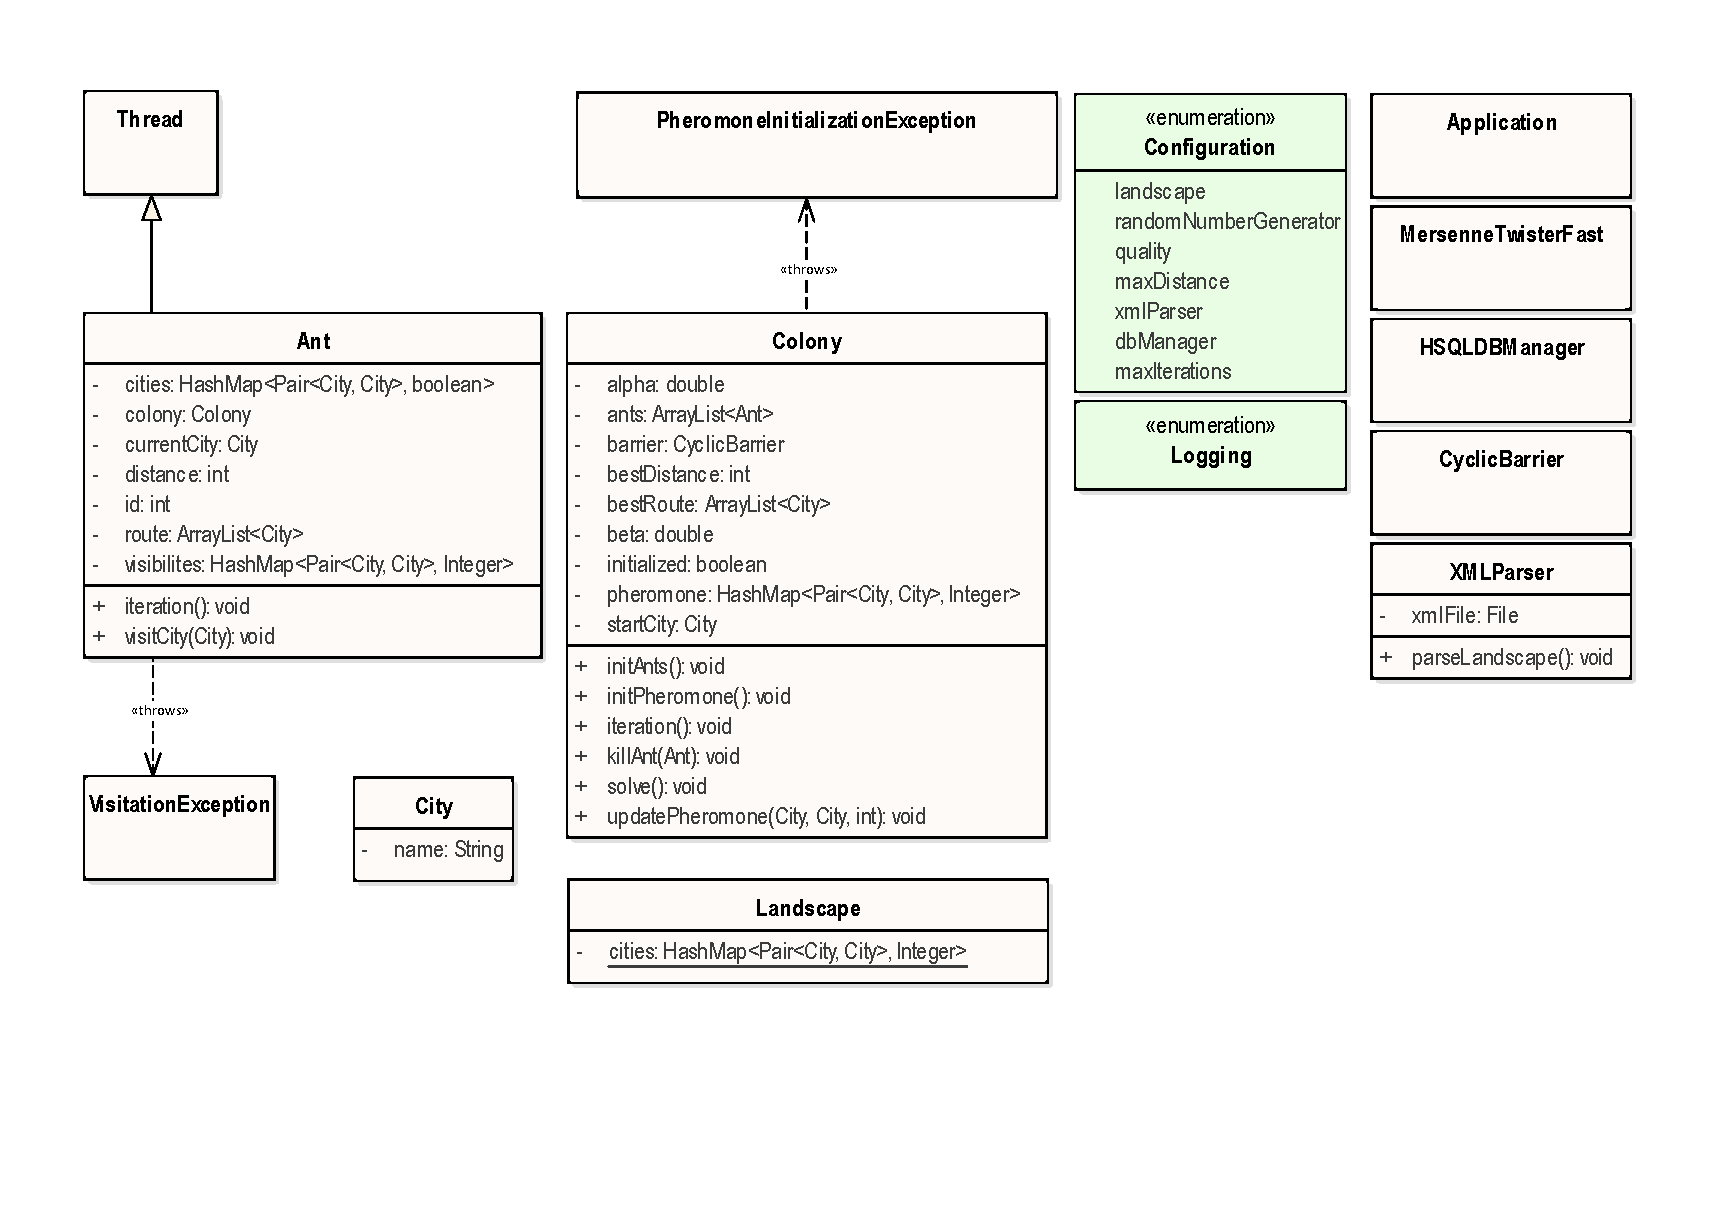
\includegraphics[width=0.9\linewidth]{images/classModel.eps}
		\caption{UML-Modellierung des Architekturentwurfs}
		\label{uml_class}
	\end{figure}

}
\section{Ausgewählte Algorithmen}{
\label{algorithms}
	Bereits vorgestellt wurden die einzelnen Bestandteile der Architektur, sowie die Architektur als Gesamtbild gezeigt. Im Folgenden sollen beispielhaft die verwendeten Algorithmen thematisch vorgestellt werden. So werden die zentralen Methoden zur Berechnung der Iterationen aus Sicht der Ameisen vorgestellt, sowie auch das Verhalten der Pheromonänderung. Zusätzlich wird die Methode zum Töten einer Ameise beschrieben, welche in so gut wie keiner Implementierung zu finden ist.
	
	\subsection{Ant - iteration()}
	In dem \ref{parameter} wurde bereits die Berechnung beschrieben, die für jede neue Streckenauswahl von den Ameisen durchgeführt werden muss. Diese Berechnung wird in der Implementierung in der Iteration der Ameisen umgesetzt. Pro Durchgang bzw. Iteration wird also jede besuchbare, angrenzende Stadt betrachtet und auf Ihre Attraktivität untersucht. Überwiegt der Pheromonwert $\tau$, welcher über Alpha gewichtet ist, über dem heuristischen Faktor $\eta$, der mit Beta verrechnet wird, so wird die bisher von der Kolonie gewählten Strecke gewählt. Diese Berechnung wird für alle Städte berechnet und dann verglichen. Die im Vergleich attraktivste Strecke wird in diesem Zusammenhang dann gewählt.
	Nachdem eine Strecke gewählt wird, verteilt die Ameise auf der Strecke ihre Pheromone indem der Kolonie ein Pheromonwert mitgeteilt wird, welcher auf den bisherigen addiert werden muss.
	
	\subsection{Colony - killAnt()}
	Ebenfalls in dem in Abbildung \ref{uml_class} gezeigten UML-Diagramm erkennbar ist, dass die Ameisenkolonie die Möglichkeit besitzt einzelne Ameisen zu "töten". 
	Diese Methode sollte in einem einwandfreiem Programm keinerlei Verwendung finden, allerdings kann man sich nicht auf eine dauerhafte fehlerfreie Implementierung verlassen. Im Bereich der Software Tests ist dies durch das Prinzip "Fehlen von Fehlern" beschrieben. Dieses sagt aus, dass erfolgreiche Tests nur bestätigen, dass keine Fehler gefunden wurden. Es kann nicht ausgesagt werden, dass keine Fehler vorliegen.\footnote{vgl. \cite{bibid}}
	
	Denn die Methode hat die Funktion, im Falle des Fehlverhaltens eine Ameise aus der Liste der aktiven Ameisen bzw. Threads zu löschen und den Thread zu stoppen.
	Genutzt werden wird diese vor allem im Bereich der aufgefangenen Fehler innerhalb der Implementierung der Ameisen. Sollte eine aufgetretene Exception schwerwiegend und unlösbar sein, wird die Applikation automatisch die Funktion aufrufen.
	
	\subsection{Colony - updatePheromone()}
	Schon mehrfach erwähnt wurden die Pheromonwerte, die Pheromonmatrix, sowie die Pheromonverteilung. All diese Begriffe sind auf die Ameisenkolonie zurückzuführen. Denn diese enthält die Pheromonmatrix, die von den Ameisen zur Berechnung der Iteration benutzt wird. Um diese aktuell zu halten wird diese von jeder Ameise nach jeder Iteration upgedatet. 
	
	Dabei wird die Funktion \textit{updatePheromone} der Kolonie aufgerufen und ein neuer Wert übergeben. Die Kolonie schreibt diesen dann in die zentrale Matrix, sodass der neue Wert bei der nächsten Iteration allen Ameisen ersichtlich ist. Durch diesen gleichzeitig und unübersichtlichen Zugriff auf die Matrix, muss diese Funktion synchronisiert ablaufen um einen Datenverlust zu verhindern.
	
}
\section{Parameterbeschreibung}{
\label{parameter}
	Die Berechnung der optimalen Wegstrecke läuft über eine Wahrscheinlichkeitsrechnung, die jeweils von den einzelnen Threads bzw. Ameisen in jeder Stadt aufs neue durchgeführt wird.
	Dabei werden die Wahrscheinlichkeiten nach folgender Formel berechnet:

	\begin{equation}\label{eq:P}
		P(s_{ij}) = \frac{\tau _{ij}^{\alpha } * \eta _{ij}^{\beta}}{\sum_{x \in  N}^{ } \tau _{ix}^{\alpha }* \eta _{ix}^{\beta}}
	\end{equation}
	\begin{conditions*}
		s & Strecke zwischen zwei Städten\\
		i & Quellstadt\\
		j & Zielstadt\\
		N & Menge der von Stadt i aus erreichbaren Städte j\\\
		$\tau$ & Pheromonwert auf der Strecke i-j\\
		$\eta$ & Heuristischer Faktor für die Strecke i-j\\
		$\alpha$, $\beta$ & Innerhalb der Applikation festgelegte Parameter\\
	\end{conditions*}
	\myequations{Formel zum Berechnen der Gewichtungen bei der Wegwahl}

	Einige der Parameter sind herleitbar, wie zum Beispiel i und j die die Städte abbilden. Ebenso is N lediglich die Menge der Städte, die eine Ameise in einer bestimmten Situation noch besuchen kann. Diese wird Menge wird über den Umstand definiert, dass bereits besuchte Städte "gesperrt" sind.
	
	Allerdings gibt es auch einige Werte, die genauer beleuchtet werden müssen. Hierbei ist von $\tau$, $\eta$, $\alpha$ und $\beta$ die Rede, welche den zentralen Bereich dieser Formel bilden. Alle vier Parameter zusammen sind ausschlaggebend dafür welche Stadt von der Ameise besucht wird. Im Folgenden werden diese einzeln erklärt und Ihre Funktion dargelegt.
	
	\subsection{Tau - $\tau$}
	Tau steht in der dargestellten Formel für den Pheromonwert für die Strecke zwischen i und j. Dieser wird von der Gesamtheit der Ameisen einer Kolonie bestimmt. Die Berechnung des Pheromonwerts wird im Kapitel \ref{algorithms} noch behandelt. Von der Ameise wird also der Wert der Strecke bestimmt und mit Eta verrechnet.
	
	\subsection{Eta - $\eta$}
	Eta steht hierbei für einen Wert der nur über Konstanten bestimmt werden kann. Hierbei wird die Länge der Strecke mit einer Konstanten verrechnet, wodurch ein Wert entsteht, der für diese Strecke konstant bleibt. Es lässt sich somit sagen, dass Eta bei einer zu Beginn normalisierten Pheromonverteilung für die Ameise attraktiver erscheint.
	
	\subsection{Alpha - $\alpha$ und Beta - $\beta$}
	Die beiden konstanten Parameter Alpha und Beta beschreiben die prozentuale Wahrscheinlichkeit, ob eine Ameise der Pheromonspur folgt oder einen neuen Pfad erkundet. Da der Alpha-Wert in Beziehung mit dem Pheromonwert steht, kann durch das Festsetzen bestimmt werden ob dieser Teil der Multiplikation höher ausfällt oder geringer. Dabei werden die Werte immer so gewählt, dass $\alpha + \beta = 1$ gilt. Dies verhindert eine unnötige Berechnung großer Zahlung und stellt trotzdem die Funktionsfähigkeit sicher.
}
\section{Umsetzung der SOLID-Prinzipien}{
	Um eine saubere und übersichtliche Implementierung gibt es heutzutage eine Vielzahl von Regelwerken, Anleitungen und Vorgaben. Eine Sammlung von Grundsätzen sind die SOLID-Prinzipien. SOLID steht für \textbf{S}ingle Responsibility, \textbf{O}pen/Closed, \textbf{L}iskov Substitution, \textbf{I}nterface Segregation und \textbf{D}ependency Inversion.
	Alle diese Eigenschaften werden im Folgenden kurz erklärt und dann ihre Verwirklichung in der Architektur gezeigt.
	
	\subsection{Single Responsibility}
	Das Single-Responsibility-Prinip umschreibt den Zustand, dass Klassen max. eine Zuständig haben sollen. Klassen dürfen nicht mehrere Aufgabengebiete gleichzeitig übernehmen, da hierdurch eine Änderung an dieser Klasse zu einer Änderung mehrerer Komponenten führt und dadurch die ganze Struktur beeinflusst werden kann.
	Stattdessen wird die Software in mehrere kleinere Klassen aufgeteilt, die jeweils einen Teil übernehmen. Hierdurch ist zum Einen die Struktur einfacherer erkennbar und nachvollziehbar, da die Klassen eindeutiger definiert sind und der Code besser zusammengefasst ist. Zum Anderen sind die Abhängigkeiten aber auch auf ein Minimum reduziert.
	
	In der vorliegenden Konzeption ist dieser Grundsatz dadurch erfüllt, dass die Berechnungslogik an die Ameisen ausgegliedert ist, welche selbst keine Manipulation vornehmen. Die Ameisenkolonie hingegen funktioniert nur als Quelle der Threads und behält einige wenige Kolonie-spezifische Attribute bereit, sonst nichts.
	Andere Anwendungen, wie das Logging, das Einlesen von Konfigurationsdateien und die Zufallszahlerzeugung wurde alle in getrennte Klassen ausgegliedert, die zentral in \textit{Configuration} initialisiert werden.
	
	\subsection{Open / Closed}
	Die Open-Closed-Eigenschaft, welche eine moderne Software besitzen muss, umschreibt den Umstand, dass ein möglichst modularer Aufbau genutzt wird. So sollen Klassen so aufgebaut sein, dass bei einer Erweiterung keine Änderung bestehenden Codes notwendig wird, sondern zum Beispiel über das Implementieren eines Interfaces die alten Strukturen genutzt werden können.
	Unterscheiden muss man hier zwischen einer Erweiterung und einer Änderung. Die Software muss nicht und soll auch nicht auf eine einfache Änderung ausgelegt sein. Der Code, welcher erfolgreich implementiert wurde, soll auch in seinem Funktionsumfang weiter genutzt werden. Die bestehenden Implementierungen müssen keine Schnittstellen zur einfach Änderung enthalten.
	
	Durch die Schlichtheit der entworfenen Architektur und den auf die Problemstellung zugeschnittenen Charakter ist eine Umsetzung des Open-Closed-Prinzips nur in geringem Umfang möglich. Alleine die Parser können hiernach umgesetzt werden, in dem ein Interface eingesetzt wird. Dadurch wird ermöglicht in Zukunft auch andere Datei-Typen akzeptieren zu können.
	In der restlichen Implementierung ist eine Umsetzung nicht hilfreich oder zweckdienlich.
	
	\subsection{Liskov Substitution}
	Die Substitutionsregel von Liskov besagt, dass es möglich sein sollte eine Klasse in einem beliebigen Aufruf auch durch eine Subklasse aus zu tauschen ohne den Programmablauf zu ändern.
	Folglich müssen entweder die Implementierung abgestimmt sein, dass ein Austauschen generell möglich ist. Dies ist aber meist nicht zweckdienlich.
	Andererseits ist es auch möglich, über eine abstrakte Klasse zu arbeiten, die für Methodenaufrufe benutzt wird. So wird der Programmablauf nicht durch unterschiedliche Klassentypen unterbrochen, sondern der Entwickler ist in der Pflicht die abstrakte Klasse entsprechend umzusetzen.
	
	Ähnlich zu der Open-Closed-Eigenschaft ist auch diese Leitlinie in dem vorliegenden Entwurf nur sehr schwierig umzusetzen. Da von einem Hineinquetschen von Regeln und Leitlinien in eine Architektur generell abzuraten ist, wurde auf eine Umsetzung der Substitutionsregel generell verzichtet.
	
	\subsection{Interface Segregation}
	Die Trennung der Interfaces zielt darauf ab, Klassen nicht dazu zu zwingen Methoden zu implementieren, die gar nicht benötigt werden. So müssen in den meisten Programmiersprachen alle Methoden eines Interfaces zwingend umgesetzt werden. Dies führt aber meist zu einer aufgeblähten Codestruktur, da unnötige Methoden implementiert werden müssen, aber nie benutzt werden.
	Indem man die Interfaces in kleine Interfaces unterteilt ist es möglich durch eine Implementierung von mehrerer Interfaces auf das gleiche Ergebnis zu kommen ohne den Zwang alle anderen Interface auch umzusetzen.
	
	Aufgrund des Mangels an Interfaces in der Codestruktur der hier behandelten Architektur ist auch diese Regel nicht umgesetzt. Sobald Interface allerdings zum Einsatz kommen, muss diese Regel umgesetzt werden.
	
	\subsection{Dependency Inversion}
	Die Abhängigkeitsumkehr-Regel besagt, dass Module auf höheren Ebenen nicht auf Module niederer Ebenen angewiesen sein dürfen. Ähnlich zu den anderen Richtlinien sollen auch hier abstrakte Klassen und Interface zur Abstraktion genutzt werden.
	Allerdings gibt es noch den Zusatz, dass Abstraktionen niemals von einer detaillierten Implementierung abhängen dürfen.

	Wie bei den anderen Interface-Umsetzungen ist auch hier eine Umsetzung nicht hilfreich bzw. möglich. Dennoch sei auch hier erwähnt, dass eine Benutzung der Regel zu einfacher zu wartenden Code führt.
}
\section{Sensitivitätsanalyse}{
	Um den Einfluss von Alpha und Beta zu verdeutlichen, folgt ein Beispiel bezogen auf die Situation einer Ameisenkolonie. In Abbildung \ref{parameter_start} zu sehen ist eine Ameisenkolonie, die neu aufgebaut wurde. Diese Kolonie hat Zugang zu zwei Nahrungsquellen: Einer Wasserquelle und einer Zuckerwasserquelle. Für die Ameisen deutlich wertvoller ist die Zuckerwasserquelle, allerdings ist diese auch weiter entfernt. Zu sehen sind auch bereits Ameisen, die auf die Nahrungssuche gehen. Hierbei ist zu beachten, dass die Ameisen im derzeitigen Zustand gleich verteilt sind.
	\begin{figure}[h]
		\centering
		\includegraphics[width=0.9\linewidth]{images/AntAlgorithm_start.png}
		\caption{Modellierung einer Ameisenkolonie mit zwei unterschiedlichen Nahrungsquellen.}
		\label{parameter_start}
	\end{figure}
	Je länger die Nahrungssuche abläuft, desto höher wird der Pheromonwert der Strecke, an deren Ende das Zuckerwasser zu finden ist. In der im vorherigen Kapitel vorgestellten Formel sind Alpha und Beta die beiden Parameter, über die bestimmt wird wie sehr der Pheromonwert gewichtet wird. 
	
	Die folgenden Beispiele basieren auf der Annahme, dass genügend Zeit vergangen ist, damit die Ameisenkolonie die Strecken ausreichend mit Pheromonen belegen konnte.
	Zusätzlich zu beachten ist, dass Alpha und Beta laut Definition der vorliegenden Architektur gemeinsam $1$ ergeben müssen.
	
	\subsection{$\alpha$ hoch - $\beta$ niedrig}
	Wird Alpha maßgeblich größer gewählt als Beta, so wird der Pheromonwert der Strecke höher gewichtet als die Länge. Auf das Beispiel angewendet bedeutet das, dass die Ameisen - wie in Abbildung \ref{parameter_a>b} - deutlich wahrscheinlicher das Zuckerwasser einsammeln. Diese Situation entspricht der Realität und ist die logischste. Denn der Pheromonwert soll ein Leitwert für die restliche Kolonie sein, welche Strecke wertvoll ist.
	\begin{figure}[h]
		\centering
		\includegraphics[width=0.7\linewidth]{images/AntAlgorithm_alphaMbeta.png}
		\caption{Modellierung der Parametereinstellung, sodass der Wert Alpha merklich größer als der von Beta ist.}
		\label{parameter_a>b}
	\end{figure}
	
	\subsection{$\alpha$ mittel - $\beta$ mittel}
	Ein Fall, der ebenso möglich ist und in einem gewissen Rahmen Sinn ergibt, ist dass die beiden Parameter Alpha und Beta gleich groß gewählt werden. Hierbei würde sich das in Abbildung \ref{parameter_a=b} ergeben. Im Gegensatz zu Abbildung \ref{parameter_a>b} ist zu erkennen, dass mehr Ameisen den kürzeren Weg zur Wasserquelle wählen. Dies liegt daran, dass der Weg dorthin kürzer ist, was durch die neue Parameterverteilung höher gewichtet wird.
	\begin{figure}[h]
		\centering
		\includegraphics[width=0.7\linewidth]{images/AntAlgorithm_alphaEbeta.png}
		\caption{Modellierung der Parametereinstellung, sodass der Wert Alpha genauso groß ist wie der von Beta.}
		\label{parameter_a=b}
	\end{figure}
	Hier lässt sich die Aussage treffen, dass das Verhalten der neuen Ameisenkolonie aus Abbildung \ref{parameter_start} - sowie auch der späteren implementierten Software - diesem Zustand stark ähnelt. In beiden Fällen ist die Gewichtung ausgeglichen. Im Fall einer normalen Ameisenkolonie liegt dies aber an der noch nicht gewichteten Pheromonmatrix, die sich erst mit der Zeit aufbaut. 
	
	\subsection{$\alpha$ niedrig - $\beta$ hoch}
	Als letztes Beispiel - und auch letzten Abschnitt - folgt das Beispiel, dass die Länge der zu wählenden Strecke deutlich höher gewichtet ist als der Pheromonwert. Dies führt, wie in Abbildung \ref{parameter_a<b} zu sehen ist, dazu, dass nur einzelne Ameisen den Weg zum wertvolleren Zuckerwasser wählen. Denn die Strecke ist hierbei länger und somit weniger attraktiv.
	\begin{figure}[h]
		\centering
		\includegraphics[width=0.7\linewidth]{images/AntAlgorithm_alphaLbeta.png}
		\caption{Modellierung der Parametereinstellung, sodass der Wert Alpha merklich kleiner als der von Beta ist.}
		\label{parameter_a<b}
	\end{figure}
	Dies hat wieder für die Ameisenkolonie eine allgemeine Folge, die sich auch auf die Software übertragen würde. Denn hier würde nur mit minimaler Wahrscheinlichkeit eine Verbesserung eintreten. Zum Einen weil die Pheromongewichtung auf dem besseren Pfad nie höher aufgebaut werden kann.\footnote{Hier sei noch erwähnt, dass alle Ameisen ihre Pheromone abgeben, sodass selbst die Ameisen auf dem Weg zum Wasser diesen Weg mit Pheromonen belegen. Dies hat den Effekt, dass durch die schiere Zahl an Ameisen dieser Weg einen höheren Pheromonwert besitzt.} Zum Anderen da eine Auswahl sowieso nur mit geringer Wahrscheinlichkeit zugunsten der Pheromonmatrix ausfallen würden.
}
\chapter{Implementierung}
\input{content/02_Implementierung/klassendiagramm.tex}
\section{Beschreibung der Implementierung}
Um die Funktionsweise der Softwarelösung zu verstehen, ist eine klare Übersicht über die einzelnen Bestandteile notwendig. Diese wird im Folgenden über ein Klassendiagramm inkl. Beschreibung gegeben. Danach werden noch die einzelnen Abschnitte in ihrer Funktion beschrieben.

\subsection{Klassendiagramm}
Bevor auf den genauen Funktionsablauf der Applikation eingegangen wird, sollte zuerst ein Überblick auf die Implementierung gegeben werden. Hierzu ist in Abbildung \ref{classDiagram} der komplette Umfang aller Klassen aufgezeigt
\footnote{Aus Gründen der Übersichtlichkeit wurden die getter- und setter-Methoden weggelassen, um die Abbildung nicht über zu dimensionieren}. Leicht erkennbar ist, dass der größte Teil der Logik innerhalb des aco-Pakets - welches unter anderem Ant und Colony enthält - stattfindet. Landscape, also die Klasse welche das \ac{TSP} beschreibt, dient nur als Schnittstelle zur Abfrage der Distanzen zwischen den Städten.

\begin{figure}[h]
	\centering
	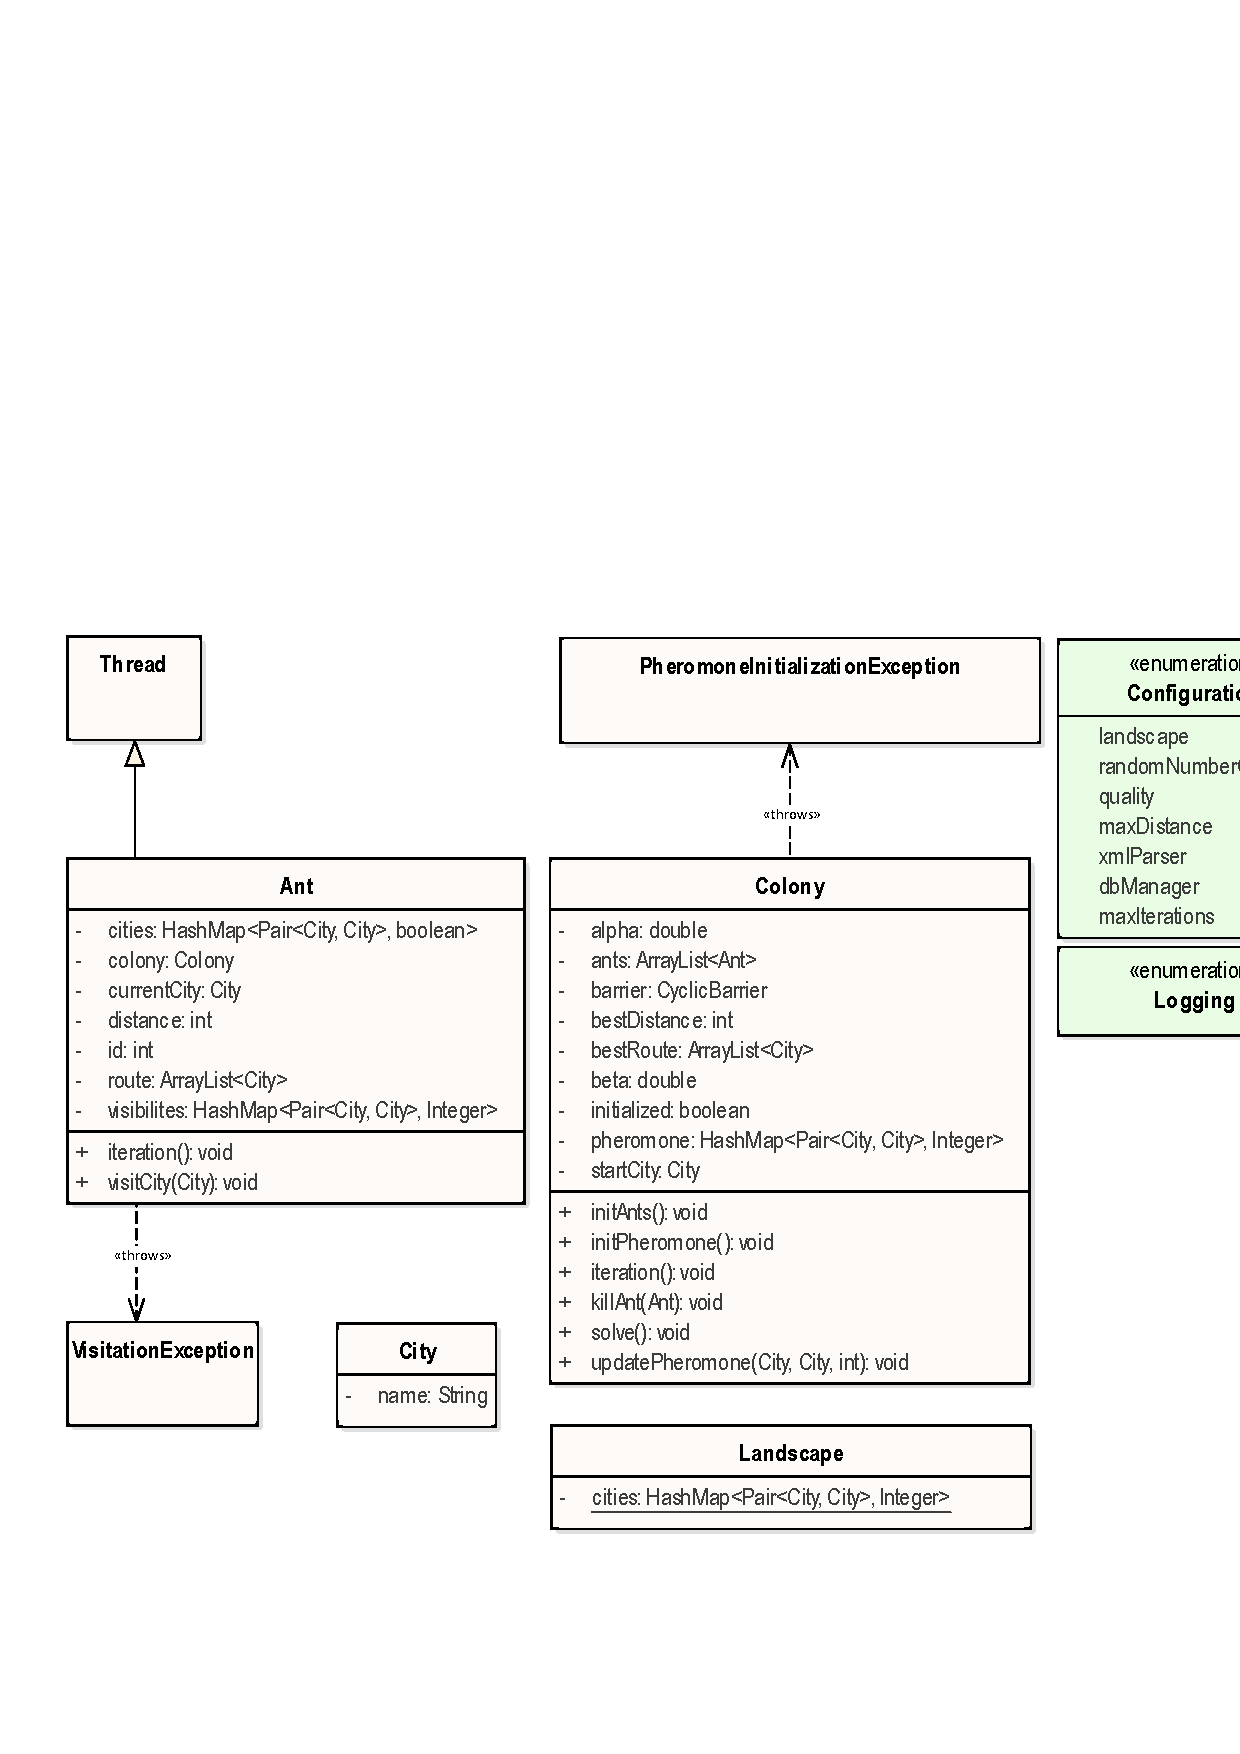
\includegraphics[width=\linewidth]{../../../01_uml/classModel.png}
	\caption{Klassendiagramm der vorliegenden Softwarelösung}
	\label{classDiagram}
\end{figure}

\subsection{Persistenz}
Um die Ergebnisse der einzelnen Generationen persistent abspeichern zu können, ohne den Speicherverbrauch des Programms ansteigen zu lassen, wird eine Datenbank-Anbindung an eine HSQLDB-Datenbank verwendet. Um die Performance möglichst hoch und den Datenbankumfang möglichst klein zu halten, werden in dieser allerdings nur zwei Tabellen erstellt und verwaltet.

\begin{figure}[h]
	\centering
	\includegraphics[width=0.4\linewidth]{images/CRC_persistenz.png}
	\caption{Modellierung der Klassen des Persistenz-Bereichs über CRC-Karten}
	\label{crcPersistenz}
\end{figure}


Zum Einen wird von jeder Generation, welche den Algorithmus durchlaufen hat, die beste Route erfasst und abgespeichert. Hierbei besteht ein Tabelleneintrag lediglich aus einer Zufalls-ID, der Route als String und der Distanz als Double. 

Zum Anderen wird eine Tabelle zur Verfolgung der Verbesserung angelegt. In der Historie wird eine Route nur dann abgespeichert, wenn diese sich im Vergleich zur vorherigen auch verbessert hat. Somit besteht diese aus den gleichen Attributen, wie die Generationen-Tabelle, mit dem Zusatz, dass auch die Generation, welche die Verbesserung verursacht hat, mit einer Ganzzahl abgespeichert wird.

\subsection{Applikation}
Dem Bereich der Applikation sind die Klassen zugeordnet, welche sich um die Initialisierung bzw. die Verwaltung von zentralen Parametern kümmern. Somit sind hier die Klassen Application, Configuration, sowie alle Implementierungen des Parser-Interfaces zu finden. In Abbildung \ref{crcApplikation} ist eine Modellierung dieser Klassen über CRC-Karten gezeigt.

Application ist beim Start des Programms dafür verantwortlich, dass alle wichtigen Instanzen korrekt initialisiert werden. Darunter fällt das Starten des Parsers, des HSQLDB-Managers, sowie der Ameisenkolonie. Sobald die Kolonie gestartet ist, ist die letzte Aufgabe der Application auf das Ende der Berechnung zu warten und dann die Datenbank wieder abbauen zu lassen.

Configuration ist als zentrale Anlaufstelle für alle Instanzen, die nur einmal benötigt werden, und alle Parameter, die mehrfach benötigt werden, gedacht. So verwaltet diese unter anderem die Gewichtung der Parameter bei der Berechnung der Wahrscheinlichkeiten. Auch wird über die Configuration der zentrale Logger bereitgestellt. Über diesen werden die Ergebnisse der Generationen erfasst bzw. auch Debug-Informationen gesammelt.

\begin{figure}[h]
	\centering
	\includegraphics[width=\linewidth]{images/CRC_applikation.png}
	\caption{Modellierung der Klassen des Applikation-Bereichs über CRC-Karten}
	\label{crcApplikation}
\end{figure}

Alle Implementierungen des Parser-Interfaces haben einen gemeinsamen Zweck: Die Landscape-Klasse - welche auch von Configuration verwaltet wird - zu konfigurieren und die Problemstellung zu generieren. Hierzu gibt es zwei Varianten: Es kann entweder eine XML-Datei erstellt werden, welche eine bestimmte Formatierung erfüllen muss. Oder aber es kann eine \ac{TSP}-Datei beigefügt werden, welche dem Standard der \ac{TSP}-Problemstellungen folgt. In beiden Fällen wird die Datei ausgelesen und die Problemstellung in die Applikation importiert, sodass die Ameisenkolonie auf dieser aufbauen kann.

\subsection{TSP}
Der \ac{TSP}-Bereich der Architektur dient zu aller erst der Verdeutlichung des Aufbaus. So soll durch die Verwendung der City-Klasse statt einfachen Integern das Verständnis gefördert werden. Innerhalb der Landscape-Instanz - welche in der Konfiguration zentral initialisiert wird -  wird die zweidimensionale Matrix der Distanzen zwischen den Städten bereit gehalten. 

Über diese Matrix kann immer zentralisiert der Wert von den Ameisen nachgefragt werden, ohne eine unnötige Berechnung durchzuführen. Ebenso fördert dieser Aufbau die Sicherung der Funktionsfähigkeit, da einfacher sichergestellt werden kann, dass die Distanzen richtig berechnet werden. Ein weiterer Vorteil ist, dass die Ameisen hier eine Liste von Nachbarn der derzeitigen Position nachfragen können, indem sie ihren derzeitigen Standort übergeben. Dies vereinfacht das Konzept bei der Berechnung innerhalb der Ameisen-Klasse.

\begin{figure}[h]
	\centering
	\includegraphics[width=\linewidth]{images/CRC_tsp.png}
	\caption{Modellierung der Klassen des \ac{TSP}-Bereichs über CRC-Karten}
	\label{crcTsp}
\end{figure}

\subsection{ACO}
Der hauptsächliche Teil der Berechnung wird innerhalb des \ac{ACO}-Bereichs durchgeführt. Denn hier befindet sich die Ameisenkolonie, als Verwaltungsorgan, und die Ameisen, welche als Threads gleichzeitig auf die Suche nach der bestmöglichen Lösung gehen.

\begin{figure}[h]
	\centering
	\includegraphics[width=\linewidth]{images/CRC_aco.png}
	\caption{Modellierung der Klassen des \ac{ACO}-Bereichs über CRC-Karten}
	\label{crcAco}
\end{figure}


Von der Kolonie werden die Ameisen insofern verwaltet, dass die Threads über diese Klasse gestartet werden, sowie hier auch die Ergebnisse abgeliefert werden. Nach jeder Generation wird innerhalb der Kolonie für jede Ameise eine Auswertung gestartet, ob die Route besser war als die derzeit beste. Sollte dies der Fall sein, wird die alte Route mit der neuen Route überschrieben.

Unabhängig davon ob eine neue beste Route gefunden wurd oder nicht, wird nach jeder Generation von Ameisen ein Update auf die Pheromonmatrix durchgeführt. Hierbei meldet jede Ameise für jeden Weg, den sie zwischen zwei Städten gegangen ist, einen Wert, welcher auf den derzeitigen Pheromonwert addiert werden soll. Hierfür iteriert eine Ameise über die Route, welche sie sich gemerkt hat, und ruft die updatePheromone-Methode der Kolonie auf, mit dem Wert $1/distance$, wobei $distance$ der Distanz zwischen der Stadt, über welche gerade iteriert wird, und der Folgestadt beträgt. 

Die restliche Berechnungsarbeit wird von den einzelnen Ameisen bzw. Threads bewältigt. Diese berechnen ab dem Startpunkt für alle möglichen Nachbarn
\footnote{Ein Nachbar ist dann erreichbar, wenn dieser noch nicht in der Route vorgekommen ist, also noch nicht besucht wurde.} einen $\lambda$-Wert\footnote{Beschrieben wurde diese Berechnung bereits in Kapitel \ref{parameter}}. 
Als nächstes werden alle $\lambda$s aufsummiert, um mit den einzelnen $\lambda$s der Städte dividiert durch die Summe die Wahrscheinlichkeit zu berechnen. Hierdurch wird beschrieben, dass Städtepaare, welche eine kurze Distanz besitzen, sowie einen hohen Pheromonwert besitzen, deutlich wahrscheinlicher besucht werden. Hierbei kann eine unterschiedliche Gewichtung vorgenommen werden, wie in Kapitel \ref{parameter} und Kapitel \ref{analyse} beschrieben wurde.

Nachdem für alle erreichbaren Städte die Wahrscheinlichkeiten berechnet wurden, wird eine Zufallszahl bestimmt. Sollte eine Wahrscheinlichkeit für eine Stadt höher sein, als die Zufallszahl so wird die Berechnung an dieser Stelle beendet und die Ameise besucht diese Stadt. Sollte diese Bedingung für keine einzelne Stadt erfüllt werden, so werden die Wahrscheinlichkeiten solange aufsummiert bis die Summe größer ist als die Zufallszahl. Die Stadt, bei welcher diese Schwelle überschritten wird, wird dann von der Ameise aufgesucht.

Sobald jede Ameise ihre Route beendet hat und wieder bei der Anfangsstadt angekommen ist, wird über die CyclicBarrier zentral eine Methode innerhalb der Kolonie angestoßen. Diese fordert nach und nach jede Ameise auf, das Ergebnis zu melden, um die Pheromonmatrix zu aktualisieren. Nachdem die Kolonie vollständig aktualisiert wurde, ist die derzeitige Generation beendet und es wird eine neue generiert und gestartet.
\input{content/02_Implementierung/erdiagramm.tex}
\input{content/02_Implementierung/komponentendiagramm.tex}
\section{Paket-Diagramm}{
	\begin{figure}
		\centering
		\includegraphics[width=0.9\linewidth]{images/packageModel.png}
		\caption{Modellierung der Software-Architektur als Paketdiagramm. Zu sehen ist der logische Aufbau der Software, sowie der Zusammenhang der einzelnen Pakete.}
	\end{figure}
	
}
\section{Perforamce-Analyse und -Optimierung}
\chapter{Evaluation der Implementierung}
\label{evaluation}
\section{Betrachtung der Auswirkung der Parametergewichtung}

\section{Auswirkung von hoher Anzahl an parallelen Threads}

\section{Verhalten bei hoher Laufzeit}
\chapter{Proof Of Concept}
\label{proofOfConcept}
\chapter{Optimierung der Softwarelösung}
\label{optimierung}
\section{Benötigter Heap-Speicher}

\section{Optimierung der Datenbankzugriffe}

\section{Ansätze zur Verbesserung der Distanzwerte}

\subsection{Verringerung der Werte innerhalb der Pheromonmatrix nach einer festen Zeit}

\subsection{Mutation der Pheromonmatrix}
\chapter{Fazit}
Ich bin ein Fazit

\backmatter

\sloppy

\cleardoublepage
\phantomsection
\addcontentsline{toc}{chapter}{Literaturverzeichnis}
\printbibliography[title=Literaturverzeichnis]

\appendix
\addchap{Anhang}
\begin{appendices}
	
	\begin{figure}[h]
		\centering
		\caption{CD mit komplettem Source-Code der Applikation, sowie einer digitalen Version dieser Arbeit}
		\label{cd_freeSpace}
	\end{figure}
	\newpage
	
	\begin{figure}[h]
		\centering
		\caption{Klassendiagramm der vorliegenden Softwarelösung}
		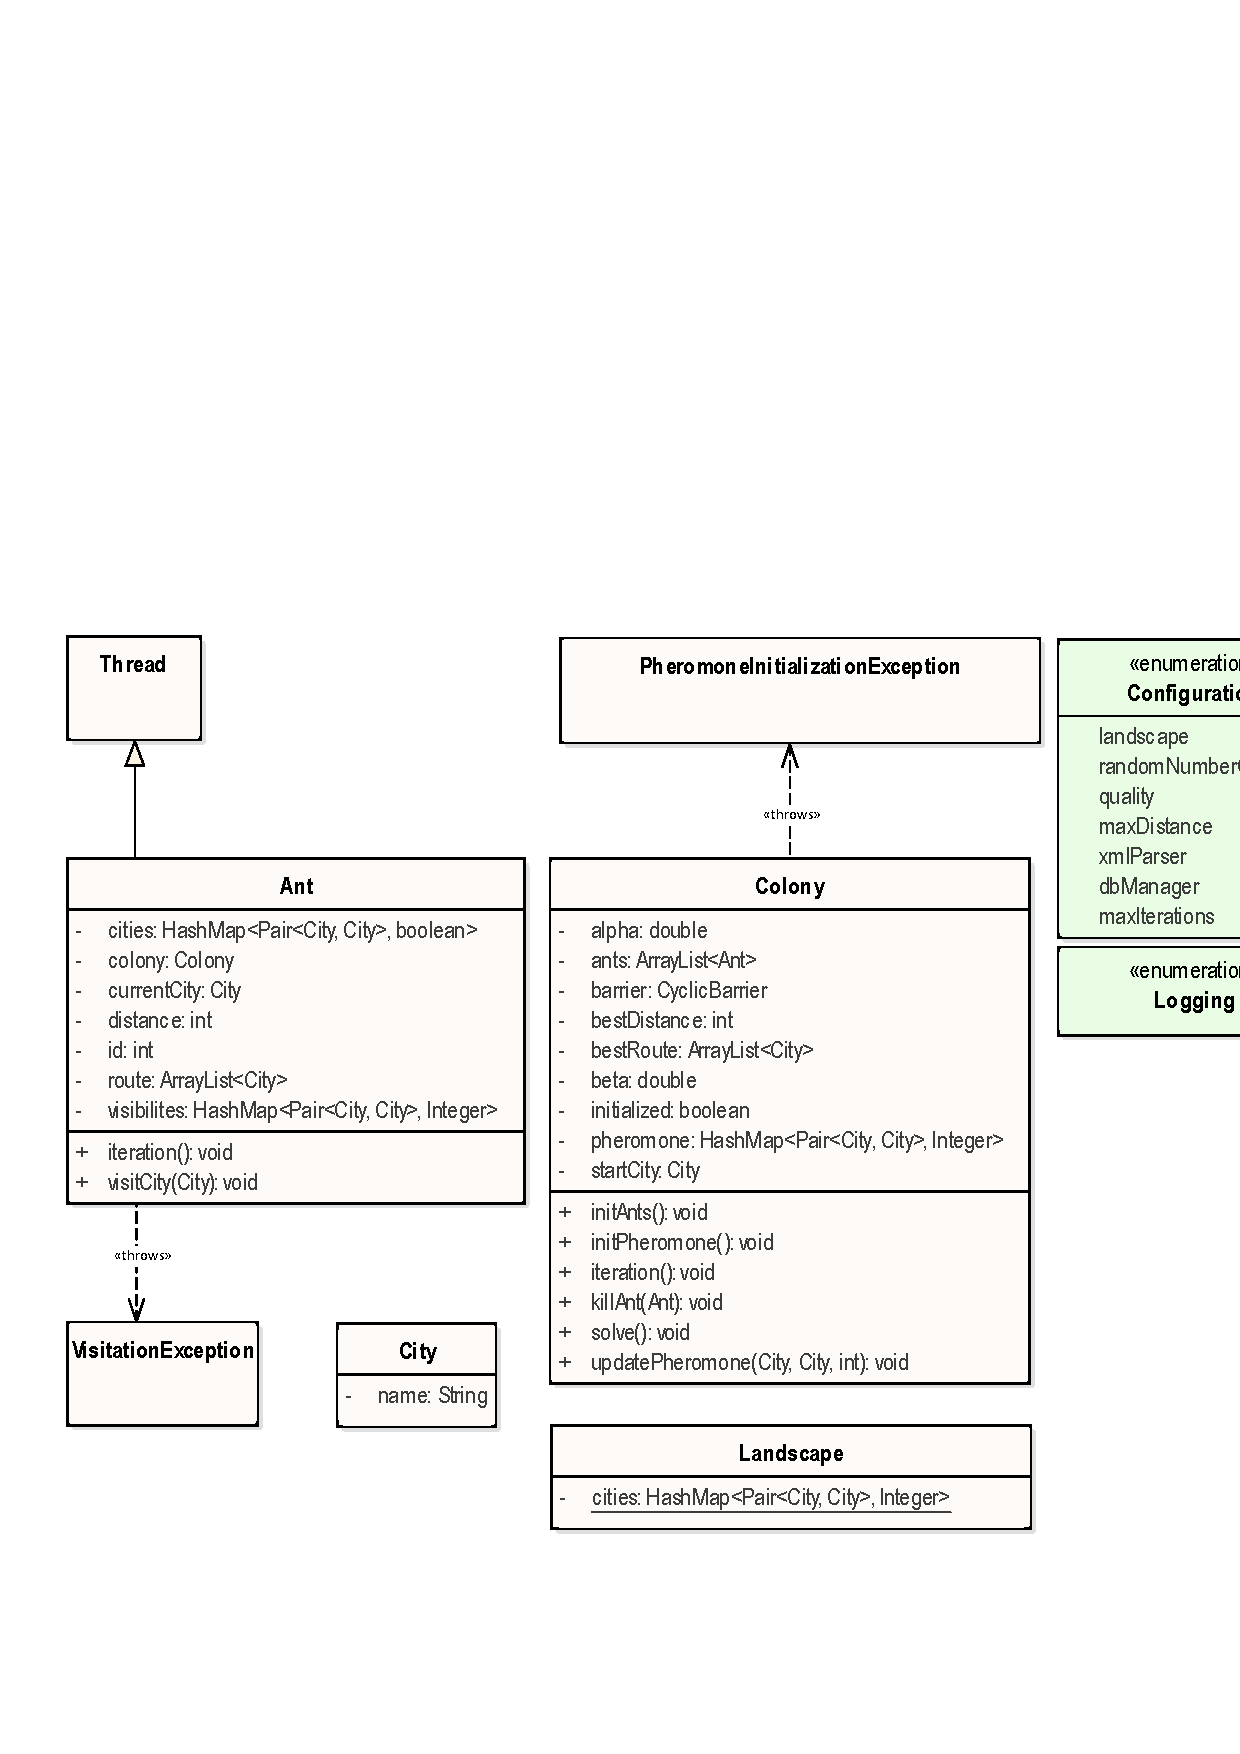
\includegraphics[width=\linewidth]{../../../01_uml/classModel.png}
		\label{classDiagram_FullSize}
	\end{figure}
	
	\begin{figure}[h]
		\centering
		\caption{Paketdiagramm der vorliegenden Softwarelösung}
		\includegraphics[width=\linewidth]{../../../01_uml/packageModel.png}
		\label{packageDiagram}
	\end{figure}

	\begin{figure}[h]
		\centering
		\caption{\acs{ER}-Diagramm der vorliegenden Softwarelösung}
		\includegraphics[width=\linewidth]{../../../01_uml/erDiagram.png}
		\label{erDiagram}
	\end{figure}

	\begin{figure}[h]
		\centering
		\caption{Testfälle der Klasse $Ant$, Seite 1}
		\includegraphics[width=\linewidth]{images/Testfaelle_Ant_Seite_1.pdf}
		\label{testAnt1}
	\end{figure}
	\begin{figure}[h]
		\centering
		\caption{Testfälle der Klasse $Ant$, Seite 2}
		\includegraphics[width=\linewidth]{images/Testfaelle_Ant_Seite_2.pdf}
		\label{testAnt2}
	\end{figure}
	\begin{figure}[h]
		\centering
		\caption{Testfälle der Klasse $Ant$, Seite 3}
		\includegraphics[width=\linewidth]{images/Testfaelle_Ant_Seite_3.pdf}
		\label{testAnt3}
	\end{figure}

	\begin{figure}[h]
		\centering
		\caption{Testfälle der Klasse $Colony$, Seite 1}
		\includegraphics[width=\linewidth]{images/Testfaelle_Colony_Seite_1.pdf}
		\label{testColony1}
	\end{figure}
	\begin{figure}[h]
		\centering
		\caption{Testfälle der Klasse $Colony$, Seite 2}
		\includegraphics[width=\linewidth]{images/Testfaelle_Colony_Seite_2.pdf}
		\label{testColony2}
	\end{figure}

	\begin{figure}[h]
		\centering
		\caption{Testfälle der Klasse $Landscape$, Seite 1}
		\includegraphics[width=\linewidth]{images/Testfaelle_Landscape_Seite_1.pdf}
		\label{testLandscape1}
	\end{figure}
	\begin{figure}[h]
		\centering
		\caption{Testfälle der Klasse $Landscape$, Seite 2}
		\includegraphics[width=\linewidth]{images/Testfaelle_Landscape_Seite_2.pdf}
		\label{testLandscape2}
	\end{figure}

	\begin{figure}[h]
		\centering
		\caption{Testfälle der Klassen von $Parser$}
		\includegraphics[width=\linewidth]{images/Testfaelle_Parser_Seite_1.pdf}
		\label{testParser1}
	\end{figure}

	\begin{figure}[h]
		\centering
		\caption{Testfälle der Klasse $HSQLDBManager$, Seite 1}
		\includegraphics[width=\linewidth]{images/Testfaelle_HSQLDB_Seite_1.pdf}
		\label{testHSQLDB1}
	\end{figure}
	\begin{figure}[h]
		\centering
		\caption{Testfälle der Klasse $HSQLDBManager$, Seite 2}
		\includegraphics[width=\linewidth]{images/Testfaelle_HSQLDB_Seite_2.pdf}
		\label{testHSQLDB2}
	\end{figure}
\end{appendices}

\end{document}